%%%%%%%%%%%%%%%%%%%%%%%%%%%%%%%%%%%%%%%%%%%%%%%%%%%%%%%%%%%%%%%%%%%%%%%%%%%%%%%%%%%%
% Document data
%%%%%%%%%%%%%%%%%%%%%%%%%%%%%%%%%%%%%%%%%%%%%%%%%%%%%%%%%%%%%%%%%%%%%%%%%%%%%%%%%%%%
\documentclass[12pt]{article} %report allows for chapters
%%%%%%%%%%%%%%%%%%%%%%%%%%%%%%%%%%%%%%%%%%%%%%%%%%%%%%%%%%%%%%%%%%%%%%%%%%%%%%%%%%%%
\usepackage{preamble}
\newcommand{\curvegamma}{\boldsymbol{\vec{\gamma}}}
\newcommand{\tangentgamma}{\boldsymbol{\dot{\vec{\gamma}}}}
\newcommand{\normalgamma}{\boldsymbol{\ddot{\vec{\gamma}}}}
%\newcommand{\forcevec}{\boldsymbol{\vec{F}}}
\newcommand{\rvec}{\boldsymbol{\vec{r}}}
\newcommand{\grad}{\boldsymbol{\vec{\nabla}}}
\newcommand{\vecfieldV}{\boldsymbol{\vec{V}}}
\newcommand{\vecfieldU}{\boldsymbol{\vec{U}}}
\newcommand{\vecfieldW}{\boldsymbol{\vec{W}}}
\newcommand{\veclaplace}{\boldsymbol{\vec{\Delta}}}
\newcommand{\vecfieldB}{\boldsymbol{\vec{B}}}
\newcommand{\vecfieldE}{\boldsymbol{\vec{E}}}
\usepackage{multicol}

\begin{document}

\begin{center}
   \textsc{\large MATH 272, Worksheet 2}\\
   \textsc{Vector fields and differential calculus of fields.}
\end{center}
\vspace{.5cm}


\begin{problem}
These same functions appeared on Worksheet 1 for which you plotted the level surfaces. Now, to analyze these functions further, compute and plot the gradient vector fields. Compare your understanding of the gradient field with the level surfaces; what is their relationship?
\begin{multicols}{2}
\begin{enumerate}[(a)]
    \item $E(x,y,z) = \frac{x^2}{25} + \frac{y^2}{16} + \frac{z^2}{9}$.
    \item $f(x,y,z) = xyz$.
    \item $g(x,y,z) = e^x-y^2-z^2$.
    \item $h(x,y,z) = \sin(x)+\cos(y)-\tanh(z)$.
    \item $p(x,y,z) = \sin^2(x)+\sin^2(y)-\frac{1}{2}\sin(z)$.
    \item $q(x,y,z) = x^2+xy+y^2+sin(yz)$.
    \item One of your own choosing.
\end{enumerate}
\end{multicols}
\end{problem}
\begin{solution}
For sake of brevity, I will compute and plot the gradients for (a), (b), and (c). 

To address the latter portion of the question, the connection between the gradients and level sets is that the gradient vector field is perpendicular to the level sets. To display this, I will plot the gradient vectors along with the surfaces. This is easiest seen with a two dimensional scalar function $f(x,y)$ and the level sets there. For example, take $f(x,y)=x^2-y^2$ then $\grad f = \begin{pmatrix} 2x \\ -2y \end{pmatrix}$ and we get the following plot.
\begin{figure}[H]
    \centering
    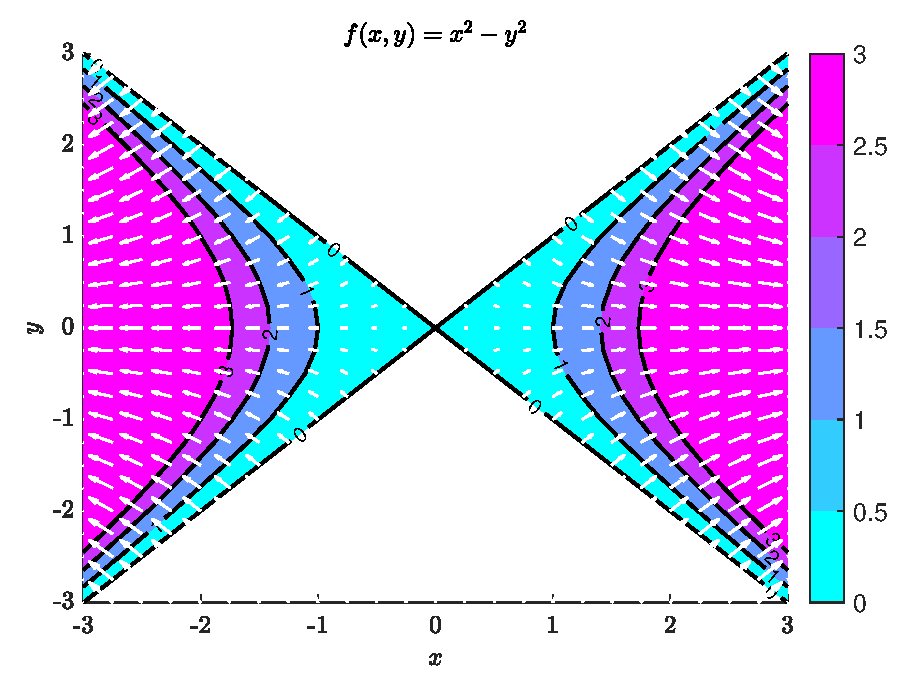
\includegraphics[width=.65\textwidth]{figures/1}
\end{figure}
One should notice how the gradient vector field is perpendicular to the level curves in this plot and point towards the direction of steepest increase for the function $f(x,y)$. This is \emph{always} the case, even in 3-dimensions; it may just be harder to visualize!
\begin{enumerate}[(a)]
    \item We have
    \[
    \grad E = \begin{pmatrix} \frac{2x}{25} \\ \frac{y}{8} \\ \frac{2z}{9} \end{pmatrix}.
    \]
    We can then plot the vector field and, for example, the level surface for $c=1$ at the same time. Notice how the gradient vector field points perpendicular to the level surface!
    \begin{figure}[H]
        \centering
        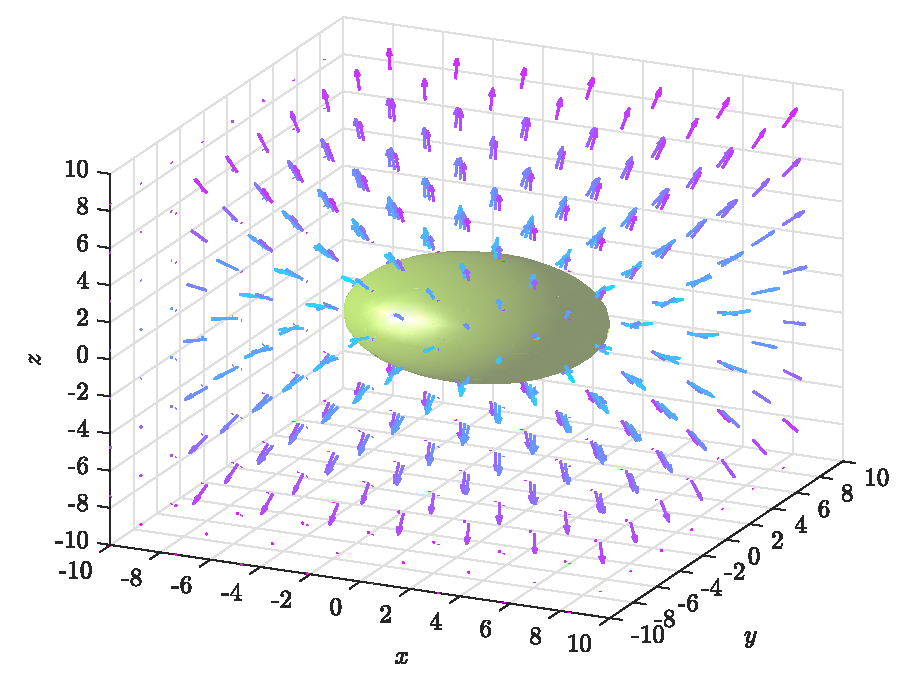
\includegraphics[width=.65\textwidth]{figures/1a}
    \end{figure}
    \item We have
    \[
    \grad f = \begin{pmatrix} yz \\ xz \\ xy \end{pmatrix}.
    \]
    We can then plot the vector field and the level surface for $c=1$ at the same time. Again, the gradient will always be perpendicular to the level sets!
    \begin{figure}[H]
        \centering
        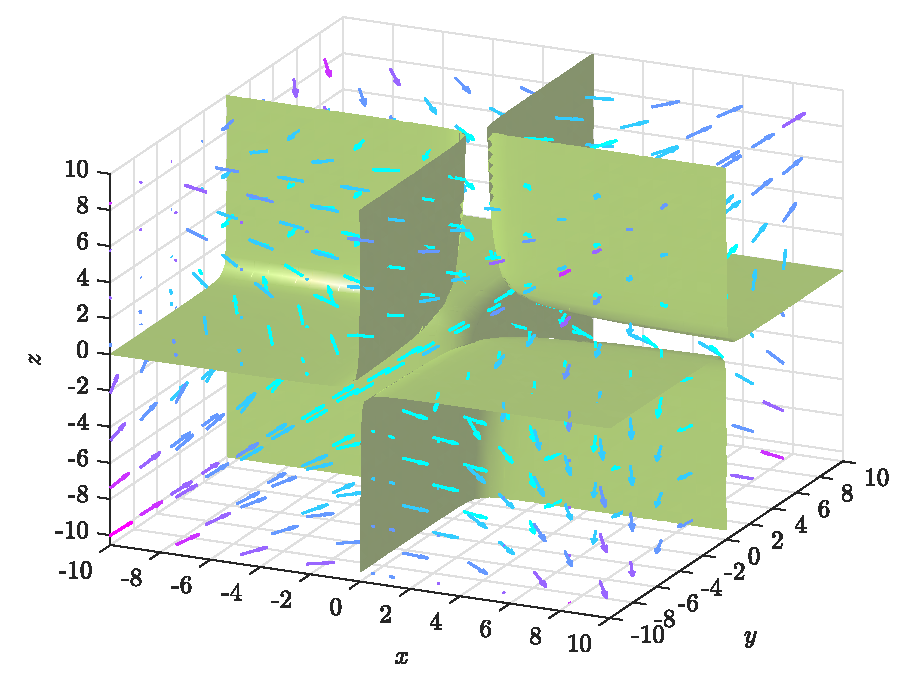
\includegraphics[width=.65\textwidth]{figures/1b}
    \end{figure}
    \item Finally, we have
    \[
    \grad g = \begin{pmatrix} e^x \\ -2y \\ -2z \end{pmatrix}.
    \]
    We can then plot the vector field and, for example, the level surface for $c=1$ at the same time. Here, it may be a bit harder to interpret this surface and the gradient.
    \begin{figure}[H]
        \centering
        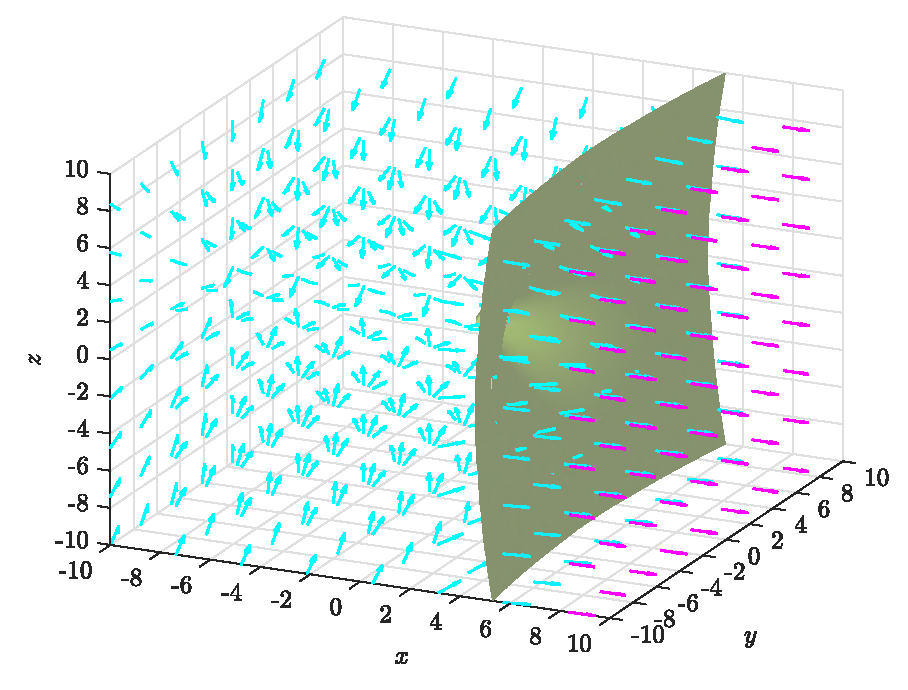
\includegraphics[width=.65\textwidth]{figures/1c}
    \end{figure}

\end{enumerate}
\end{solution}

\newpage
\begin{problem}
Let $h(x,y)$ be the height of a sheet above the $xy$-plane at the point $(x,y)$. Then, the level sets of $h$ are exactly the lines you find in a topographic map. Below is a map of White River National Forest, CO including Snowmass Peak. 
\begin{enumerate}[(a)]
    \item Determine the level set (possibly multiple curves) for $h(x,y)=12,000$.
    \item In the coordinates of this map, the town of Crystal and the famous Crystal Mill is located roughly at $x=18$, $y=25.5$. Locate this point and describe the local geometry (e.g., where the steep and shallow gradients are, which way the river should flow).
    \item Sheep Mountain is located at roughly $x=16.5$ and $y=26$. What is the max elevation of Sheep Mountain?
    \item You want to hike to Snowmass Peak (roughly $(21.5,32)$) because you are very brave. Assuming you are dropped off at Lead King Basin (roughly $(20,28)$). Assuming you can hike over any terrain (including water if need be), can you find a path that follows the steepest gradient from Lead King Basin to Snowmass Peak?
    \item Locate the flattest area that you can.
    \item Plot gradient vectors at each point on the grid.
    \item Follow Schofield Pass starting from roughly $(22.5,19)$. How much elevation gain and loss do you experience over this curve? Can you think of how we could represent this via integration? (\emph{Hint: you may be able to use both $h$ and $\grad h$ to compute this in different ways; we'll return to this idea in the future.})
\end{enumerate}
\begin{figure}[H]
    \centering
    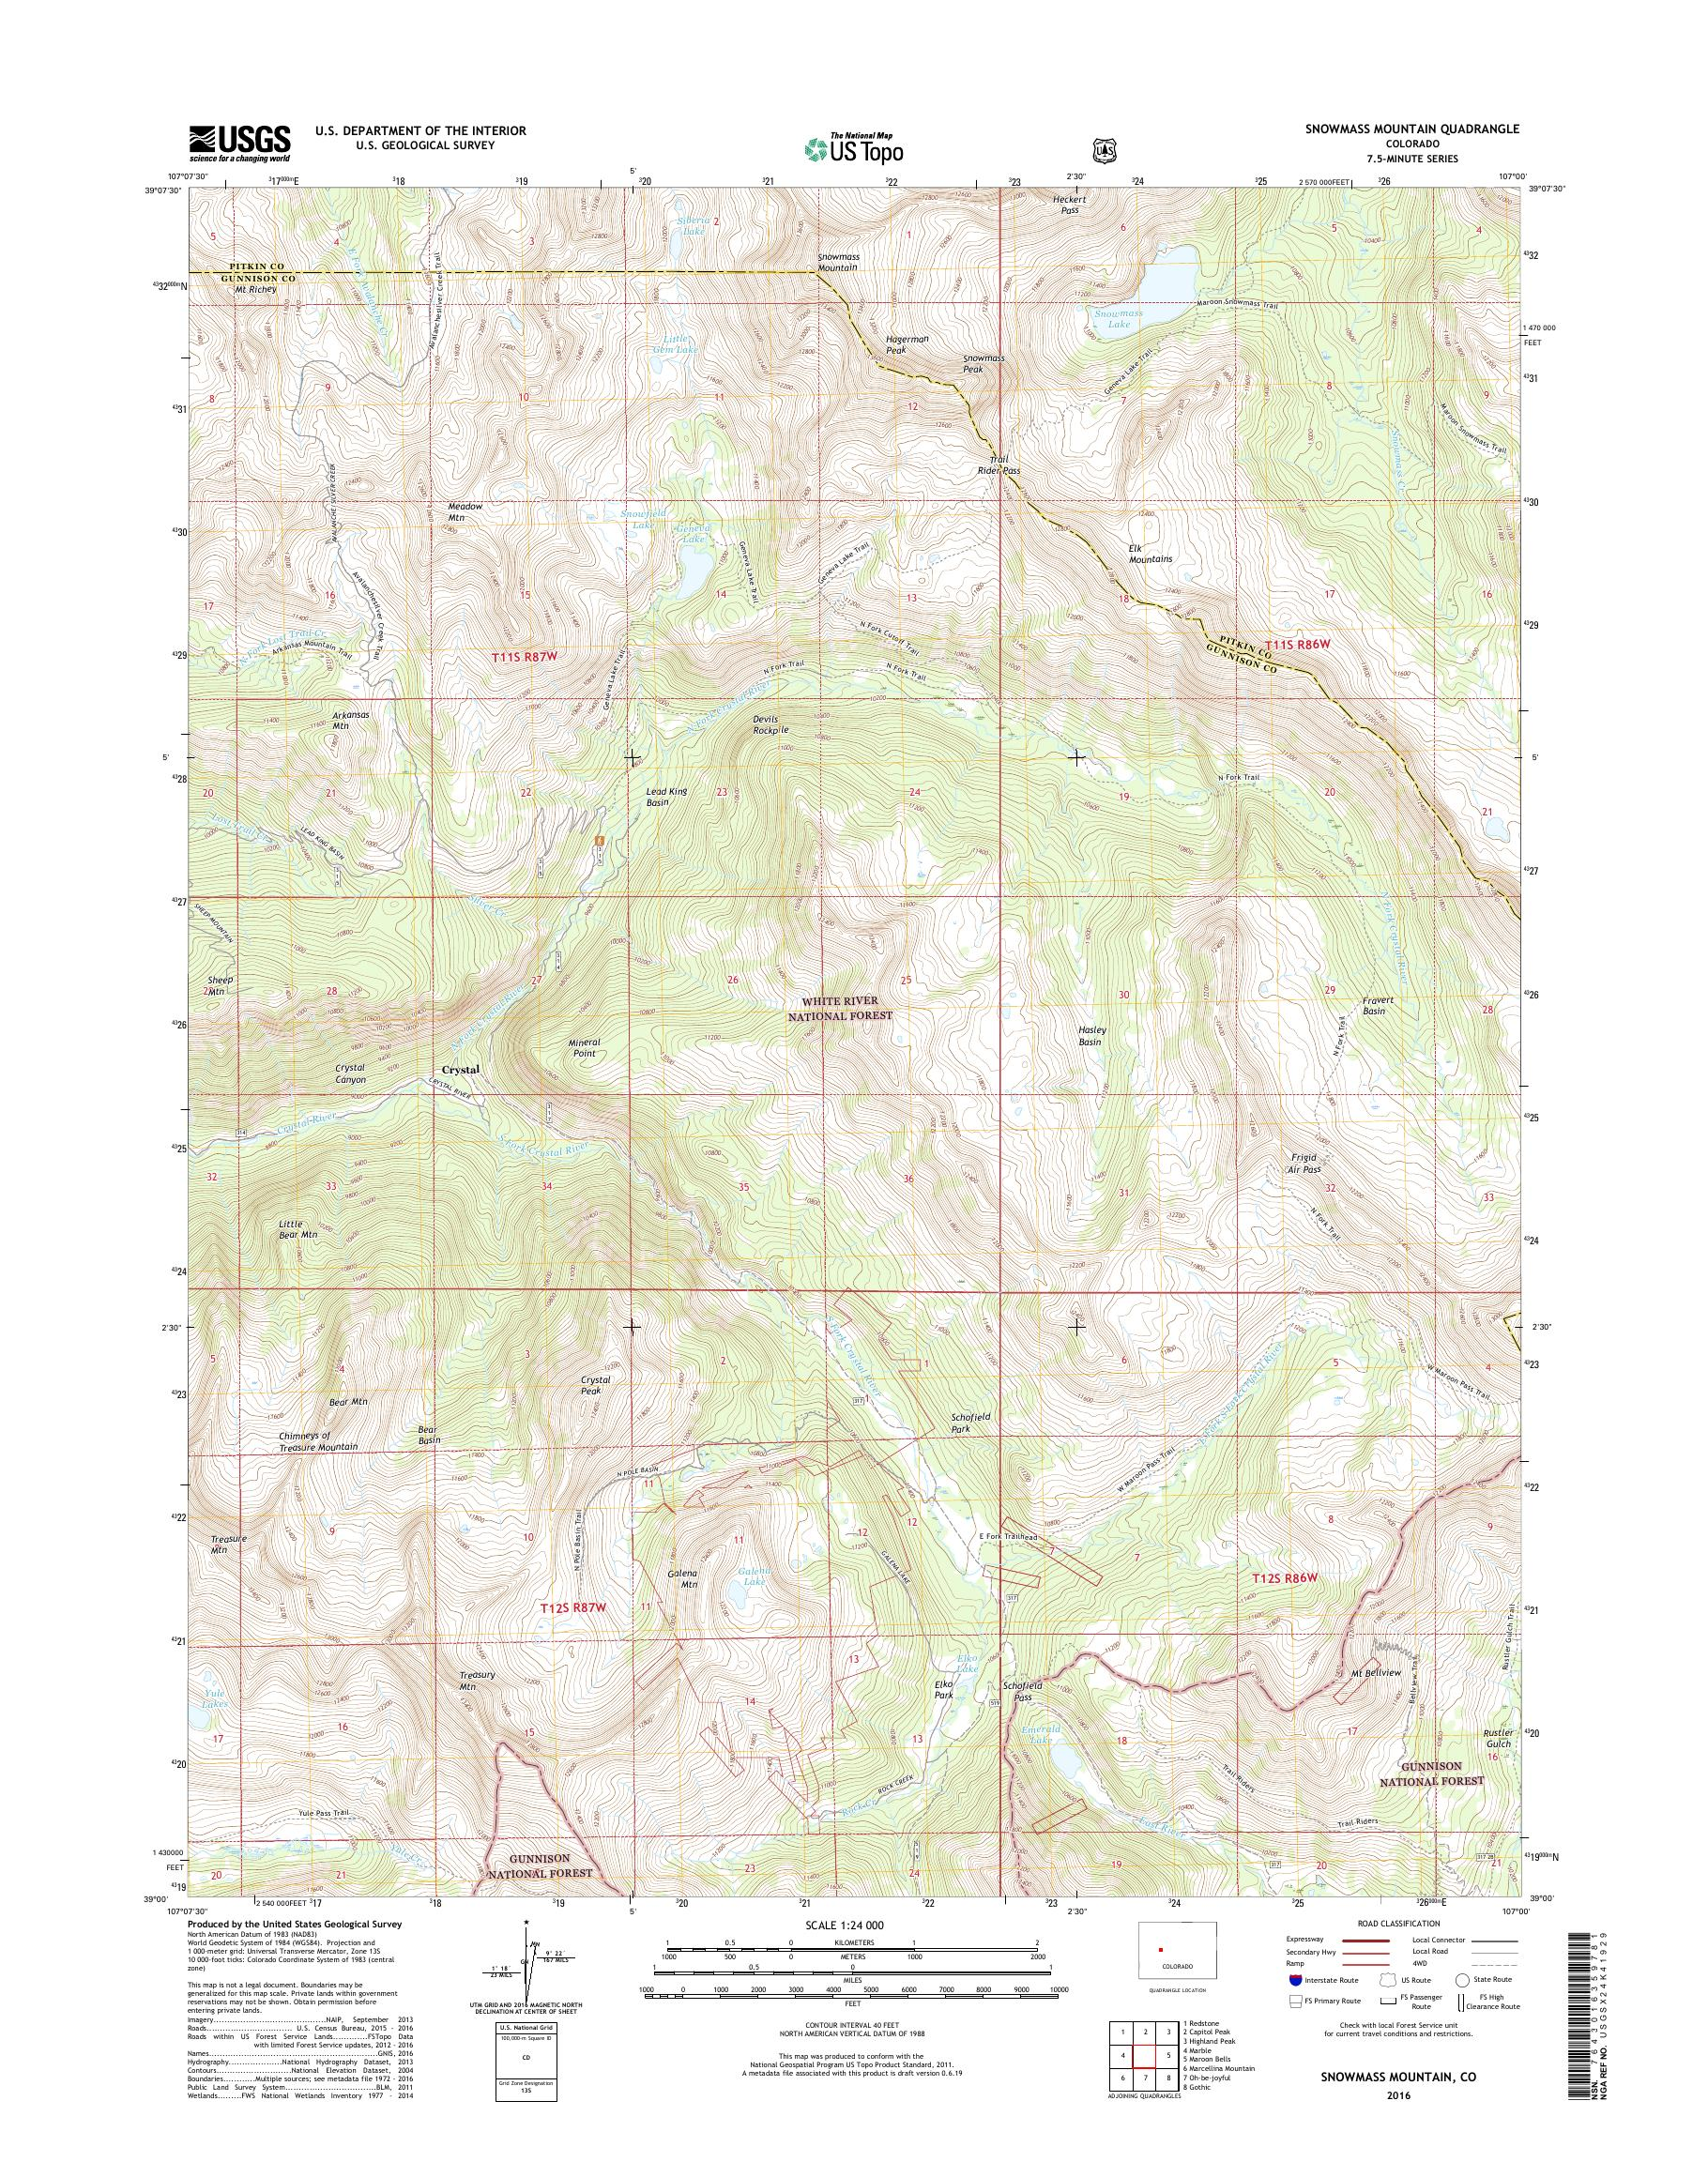
\includegraphics[width=1.1\textwidth]{figures/snowmass_topo.jpg}
\end{figure}
\end{problem}
\begin{solution}
Let me think of a good way to do this...
\end{solution}


\newpage
\begin{problem}
Plot the following vector fields.
\begin{multicols}{2}
\begin{enumerate}[(a)]
    \item $\vecfieldU(x,y,z) = \begin{pmatrix} xyz \\ xyz \\ xyz \end{pmatrix}$.
    \item $\vecfieldV(x,y,z) = \begin{pmatrix} e^{x+y+z} \\ e^{x+y+z} \\ e^{x+y+z} \end{pmatrix}$.
    \item $\vecfieldW(x,y,z) = \begin{pmatrix} x \sin(y) \\ x \cos(y) \\ xz \end{pmatrix}$.
    \item $\forcevec(x,y,z) = \begin{pmatrix} 5 + yz \\ -5 -xz \\ xy \end{pmatrix}$.
\end{enumerate}
\end{multicols}
\end{problem}
\begin{solution}
\begin{enumerate}[(a)]
    \item Here is the vector field $\vecfieldU$.
    \begin{figure}[H]
        \centering
        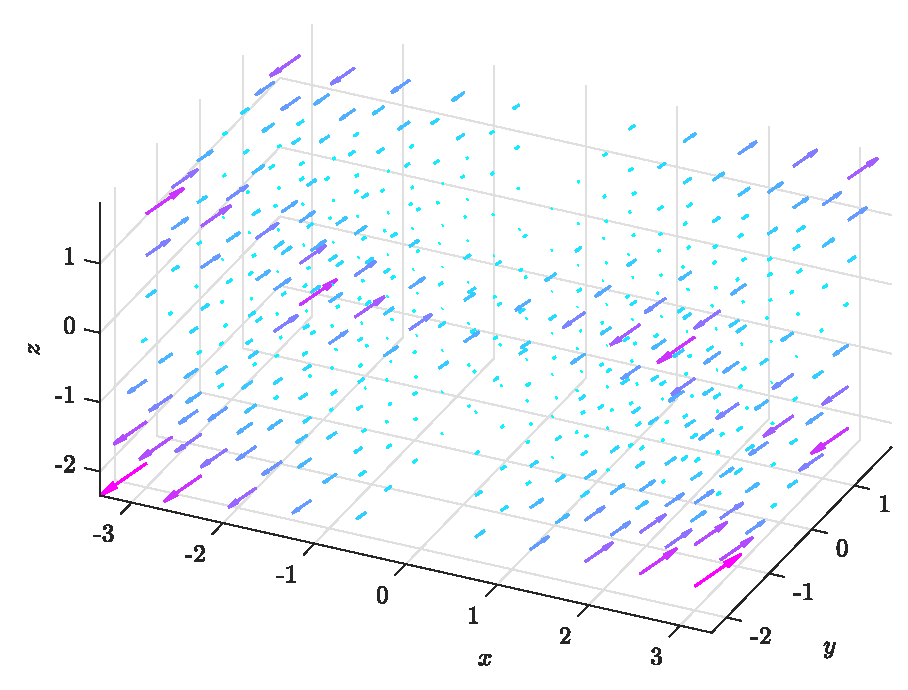
\includegraphics[width=.65\textwidth]{figures/2a}
    \end{figure}
    \item Here is the vector field $\vecfieldV$. Note that the vectors are very small in magnitude when $x,y$, and $z$ are negative. The vectors quickly grow in length as $x,y$, and $z$ increase.
    \begin{figure}[H]
        \centering
        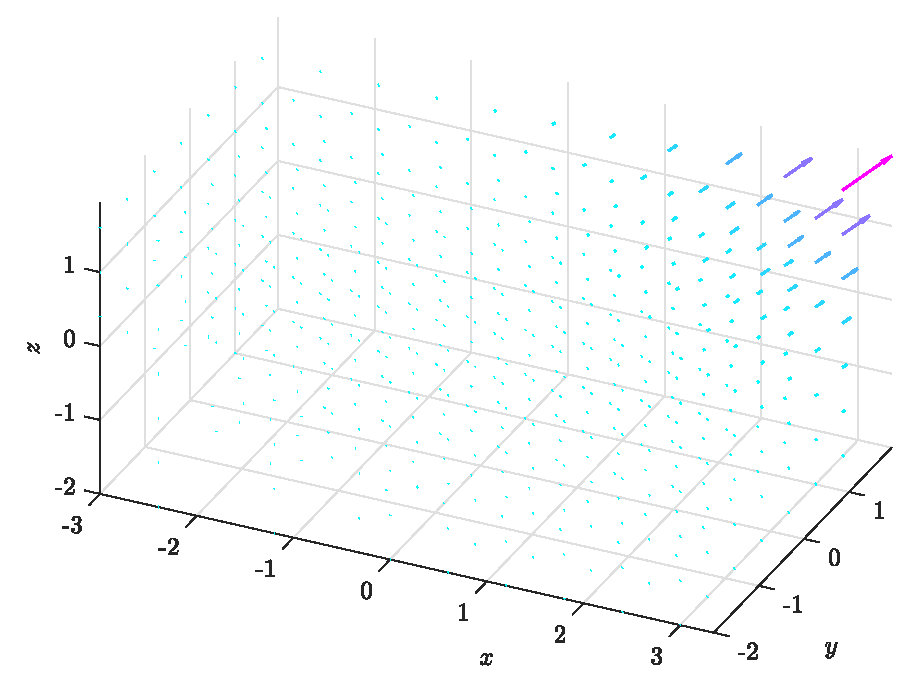
\includegraphics[width=.65\textwidth]{figures/2b}
    \end{figure}
    \item Here is the vector field $\vecfieldW$.
    \begin{figure}[H]
        \centering
        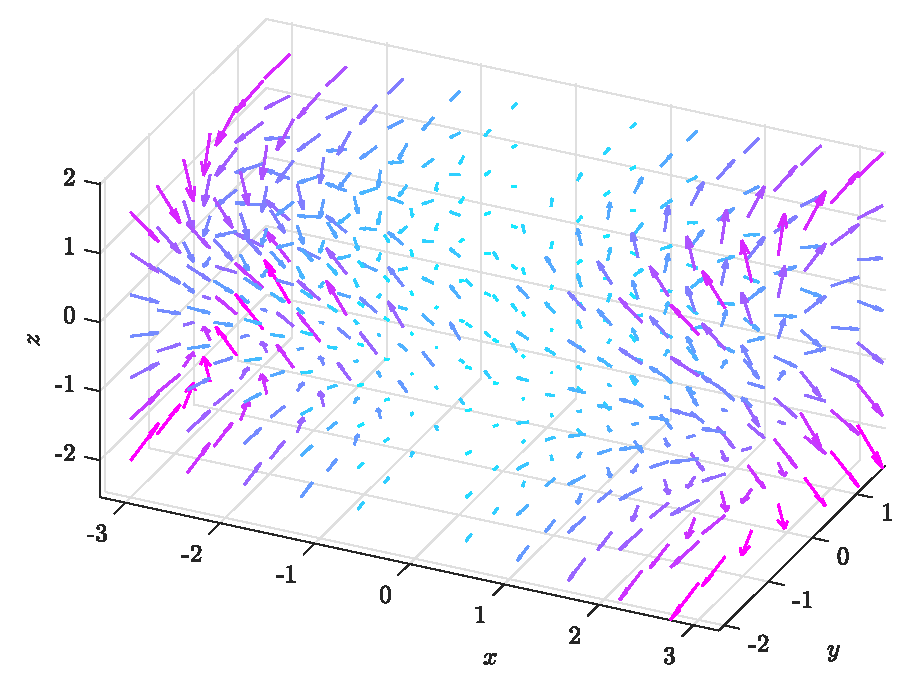
\includegraphics[width=.65\textwidth]{figures/2c}
    \end{figure}
    \item Here is the vector field $\forcevec$.
    \begin{figure}[H]
        \centering
        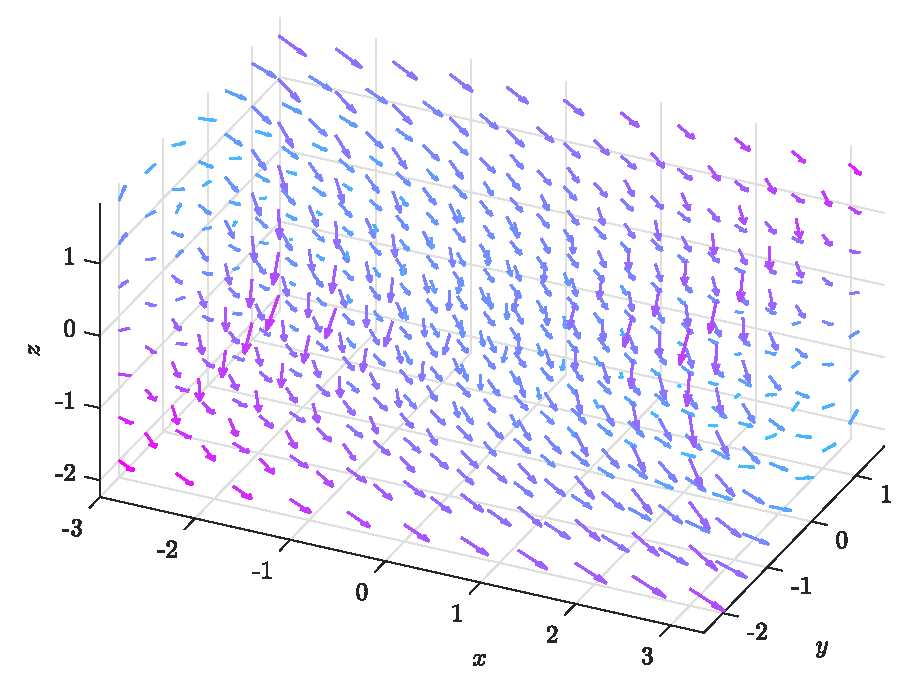
\includegraphics[width=.65\textwidth]{figures/2d}
    \end{figure}
\end{enumerate}
\end{solution}

\newpage
\begin{problem}
Compute the divergence and curl of the vector fields in Problem 3.
\end{problem}
\begin{solution}
\begin{enumerate}[(a)]
    \item We have
    \[
    \grad \cdot \vecfieldU = xy + xz + yz,
    \]
    and
    \[
    \grad \times \vecfieldU = \begin{pmatrix} x(z-y) \\ y(x-z) \\ z(y-x) \end{pmatrix}.
    \]
    \item We have
    \[
    \grad \cdot \vecfieldV = 3e^{x+y+z},
    \]
    and
    \[
    \grad \times \vecfieldV = \begin{pmatrix} 0 \\ 0 \\ 0 \end{pmatrix}.
    \]
    \item We have
    \[
    \grad \cdot \vecfieldW = -x\sin(y)+\sin(y)+x,
    \]
    and
    \[
    \grad \times \vecfieldW = \begin{pmatrix} 0 \\ -z \\ -(x-1)\cos(y) \end{pmatrix}.
    \]
    \item We have
    \[
    \grad \cdot \forcevec = 0,
    \]
    and
    \[
    \grad \times \forcevec = \begin{pmatrix} 2x \\ 0 \\ -2z \end{pmatrix}.
    \]
\end{enumerate}
\end{solution}

\newpage
\begin{problem}
Given a function, a vector, and a point, compute the directional derivatives in the direction of the given vector at that point.
\begin{enumerate}[(a)]
    \item $f(x,y)=x^2/y$, $\vecu = 3\xhat -\yhat$, and $(x,y)=(2,2)$.
    \item $g(x,y,z)=x\cos(yz^2)$, $\vecv = \frac{1}{2}\xhat + \frac{1}{2} \yhat + \zhat$, and $(x,y,z)=(0,-1,2)$.
\end{enumerate}
\end{problem}
\begin{solution}
\begin{enumerate}[(a)]
    \item First, we have
    \[
    \grad f = \begin{pmatrix} \frac{2x}{y} \\ \frac{-x^2}{y^2} \end{pmatrix},
    \]
    so at the given point we get
    \[
    \grad f(2,2) = \begin{pmatrix} 2 \\ -1 \end{pmatrix}.
    \]
    Then, we normalize $\vecu$ to get a direction vector by
    \[
    \unitvec = \frac{1}{|\vecu|} \vecu = \begin{pmatrix} \frac{3}{\sqrt{10}} \\ -\frac{1}{\sqrt{10}} \end{pmatrix}.
    \]
    Thus, the directional derivative is
    \[
        \boxed{\unitvec \cdot \grad f(2,2) = \frac{7}{\sqrt{10}} .}
    \]
    \item We simply repeat this process just for the scalar field $g$ now. So,
    \[
    \grad g = \begin{pmatrix} \cos(yz^2) \\ -xz^2 \sin(yz^2) \\ - 2xyz\sin(yz^2) \end{pmatrix},
    \]
    so at the given point we get
    \[
    \grad f(0,-1,2) = \begin{pmatrix} \cos(-5) \\ 0 \\ 0 \end{pmatrix}.
    \]
    Then, we normalize $\vecv$ to get a direction vector by
    \[
    \unitvec = \frac{1}{|\vecv|} \vecv = \begin{pmatrix} \frac{1}{\sqrt{6}} \\ \frac{1}{\sqrt{6}} \\ \sqrt{\frac{2}{3}} \end{pmatrix}.
    \]
    Thus, the directional derivative is
    \[
        \boxed{\unitvec \cdot \grad g(0,-1,2) = \frac{\cos(-5)}{\sqrt{6}} .}
    \]
\end{enumerate}
\end{solution}

\newpage
\begin{problem}
    Give a physical argument for why the field $\vecfieldU = \begin{pmatrix} 0 \\ x \\ 0 \end{pmatrix}$ has nonzero curl everywhere where $x\neq 0$. Reason why the direction of the curl is solely along the $z$-axis.  Do this \underline{without} computing the curl.
\end{problem}
\begin{solution}
Let us take a look at the vector field.
\begin{figure}[h]
    \centering
    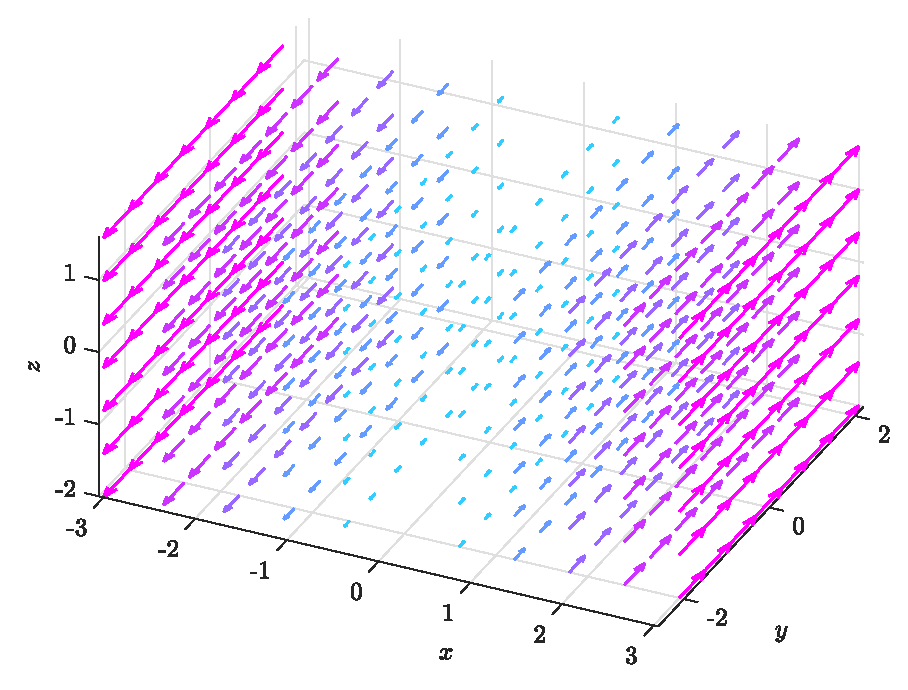
\includegraphics[width=.65\textwidth]{figures/6}
\end{figure}
If we pay close attention to this field, we notice that the vector field has some symmetry to it. For example, if we move solely in the $y$ or the $z$ directions, the field does not change. The field only changes if the $x$ position changes. So, if we were to take a small rod and place the rod so that it extends into the $x$-direction (it can have a $y$ or $z$ component as well, but it \emph{must} have some $x$ component), then the rod will rotate about the $z$-axis. Thus, we can realize the curl must be along the $z$-axis. 

Indeed, if we compute the curl if this field we find
\[
\grad \times \vecfieldU = \begin{pmatrix} 0 \\ 0 \\ 1 \end{pmatrix}.
\]
\end{solution}

\newpage
\begin{problem}
    Give a physical argument why the field $\vecfieldV = \begin{pmatrix} x \\ 0 \\ 0 \end{pmatrix}$ has nonzero divergence everywhere where $x\neq 0$. Reason why the divergence is a scalar quantity as opposed to a vector quantity. Do this \underline{without} computing the curl.
\end{problem}
\begin{solution}
Let us take a look at the vector field.
\begin{figure}[h]
    \centering
    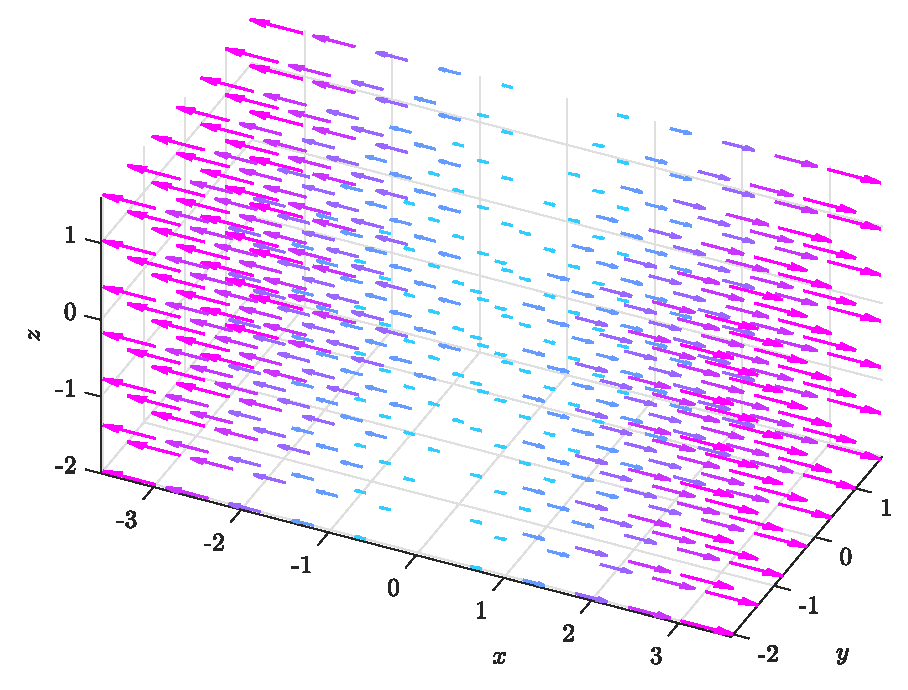
\includegraphics[width=.65\textwidth]{figures/7}
\end{figure}
Once again, we notice that this vector field has the same symmetry to it; if we move solely in the $y$ or the $z$ directions, the field does not change and the field only changes if the $x$ position changes. If we take a small point particle and place it somewhere with a positive $x$-coordinate, then the particle will accelerate in the $x$ direction. Thus, there must be some divergence.

Indeed, if we compute the divergence if this field we find
\[
\grad \cdot \vecfieldV = 1.
\]
\end{solution}

\newpage
\begin{problem}
Compute the Laplacian of the following fields.
\begin{multicols}{2}
\begin{enumerate}[(a)]
    \item $f(x,y) = (x+y)^2$
    \item $g(x,y) = (x+y)e^{x^2+y^2}$.
    \item $\vecfieldU = \begin{pmatrix} \cos(x)\cos(y)\cos(z) \\ \sin(x)\sin(y)\sin(z) \\ xyz \end{pmatrix}$.
    \item $\vecfieldV = \begin{pmatrix} \frac{y}{z} \\ \frac{x}{z} \\ \frac{x}{y} \end{pmatrix}$.
\end{enumerate}
\end{multicols}
\end{problem}
\begin{solution}
\begin{enumerate}[(a)]
    \item Explicitly, we have
    \[
    \frac{\partial^2f}{\partial x^2} = 2 \qquad \textrm{and} \qquad \frac{\partial^2f}{\partial y^2} = 2.
    \]
    Thus,
    \[
    \boxed{\Delta f = \frac{\partial^2f}{\partial x^2} + \frac{\partial^2f}{\partial y^2} = 4.}
    \]

    \item More quickly this time, we have
    \[
        \boxed{\Delta g = 4e^{x^2+y^2}\left(x^2+x^2y+x(y^2+2)+y(y^2+2)\right).}
    \]

    \item Recall the formula for the vector Laplacian is
    \[
    \veclaplace \vecfieldU = \grad (\grad \cdot \vecfieldU) - \grad \times (\grad \times \vecfieldU).
    \]
     We first compute the divergence and curl of $\vecfieldU$ to get
    \[
    \grad \cdot \vecfieldU = xy - \sin(x)\cos(y)(\cos(z)-\sin(z)
    \]
    and
    \[
    \grad \times \vecfieldU = \begin{pmatrix} xz - \sin(x)\sin(y)\cos(z) \\ -\cos(x)\cos(y)\sin(z) -yz \\ \cos(x)\sin(y)(\sin(z)+\cos(z)) \end{pmatrix}.
    \]
    Then,   
    \[
    \grad (\grad \cdot \vecfieldU) = \begin{pmatrix} (y-\cos(x)\cos(y))(\cos(z)-\sin(z)) \\ \sin(x)\sin(y)(\cos(z)-\sin(z))+x \\ \sin(x)\cos(y)(\sin(z)+\cos(z)) \end{pmatrix}
    \]
    and
    \[
    \grad \times (\grad \times \vecfieldU) = \begin{pmatrix} \cos(x)\cos(y)(\sin(z)+2\cos(z))+y \\ 2\sin(x)\sin(y)\sin(z)+\sin(x)\sin(y)\cos(z)+x \\ \sin(x)\cos(y)(\sin(z)+\cos(z)) \end{pmatrix}
    \]
    Thus,
    \[
    \veclaplace \vecfieldU = \textrm{This took me quite a while...}
    \]

    \item Let us compute the vector Laplacian of $\vecfieldV$ now. Again,
    \[
        \grad \cdot \vecfieldV = 0
    \]
    and
    \[
        \grad \times \vecfieldV = \begin{pmatrix} x\left(\frac{1}{z^2}-\frac{1}{y^2} \right) \\ \frac{-y}{z^2}-\frac{1}{y} \\ 0 \end{pmatrix}.
    \]
    Thus, we need to just compute $\grad \times (\grad \times \vecfieldV)$
    \[
        \grad \times (\grad \times \vecfieldV) = \begin{pmatrix} -\frac{2y}{z^3} \\ -\frac{2x}{z^3} \\ -\frac{2x}{y^3} \end{pmatrix}.
    \]
    Thus,
    \[
    \veclaplace \vecfieldV = \begin{pmatrix} \frac{2y}{z^3} \\ \frac{2x}{z^3} \\ \frac{2x}{y^3} \end{pmatrix}
    \]
    
\end{enumerate}
\end{solution}

\newpage
\begin{problem}
    Suppose that $\vecfieldE = \grad \phi$ for some scalar field $\phi$ (as in the static Maxwell's equations).  Explain why if $\vecfieldE$ is divergence free (i.e., if $\grad \cdot \vecfieldE=0$) that $\veclaplace \vecfieldE = \zerovec$.
\end{problem}
\begin{solution}
    Since $\vecfieldE=\grad \phi$ we can note that $\grad \times \vecfieldE = \zerovec$ since gradient fields have no curl (i.e., $\grad \times \grad \phi = \zerovec$, which occurs in a vacuum). Then, we can put
    \[
    \veclaplace \vecfieldE = \grad (\grad \cdot \vecfieldE) - \underbrace{\grad \times (\grad \times \vecfieldE)}_{=0}.
    \]
    So, if $\grad \cdot \vecfieldE = 0$ as well, then 
    \[
    \veclaplace \vecfieldE = \zerovec.
    \]
\end{solution}

\newpage
\begin{problem}
    One of Maxwell's equations states for a magnetic field $\vecfieldB$ that
    \[
    \grad \cdot \vecfieldB = 0,
    \]
    is an identity.  Does this mean that $\veclaplace \vecfieldB = 0$? 
\end{problem}
\begin{solution}
    It is tempting to believe this based on the previous problem, but this is not necessarily true. It is, however, true when $\vecfieldB$ has no curl (e.g., this will be the case if $\vecfieldB = \grad \phi$ as in the previous problem, but this is also not the \emph{only} possibility).  Writing out the Laplacian yields   
    \[
    \veclaplace \vecfieldB = \underbrace{\grad(\grad \cdot \vecfieldB)}_{=0}- \grad \times (\grad \times \vecfieldB),
    \]
    and we can see that $\grad \times (\grad \times \vecfieldB)$ would also have to be zero which may not be the case. In fact, in Maxwell's equations, $\grad \times \vecfieldB$ is related to the time derivative of the electric field $\vecfieldE$. When we take the curl again, and apply some identities, we get the equations for light waves in terms of the electromagnetic fields by
    \[
        \frac{1}{c^2} \frac{\partial^2 \vecfieldE}{\partial t^2} - \veclaplace \vecfieldE = \zerovec,
    \]
    and
    \[
        \frac{1}{c^2} \frac{\partial^2 \vecfieldB}{\partial t^2} - \veclaplace \vecfieldB = \zerovec.
    \]
    Without this structure of the Laplacian, we would not see light. Be careful to understand how the vector Laplacian behaves!
\end{solution}

\end{document}
